\chapter{Appendix D: Supplementary Neuromechanical Verification}\label{app:simulation_verification}
\graphicspath{{../Figures/95-AppendixD/}{figs/95-AppendixD/}}

This appendix supplies supporting model records and evaluation sets for Chapter~\ref{ch:sns}. It separates implementation checks, gait comparisons, pathway-removal tests, and spiking conversions because they test different claims. Neuron equations and calibration tables are provided in Appendix~\ref{app:neuron_equations}.

\section{Model Construction and Recording}

The archived AnimatLab projects provide reference circuits for implementation comparisons. Figure~\ref{fig:animatlab_controller_motifs} shows their neural organization. A later reorganized bilateral project added commissural and biarticular pathways; it ran headless but latched under the tested drives. That assembly result is not evidence of stepping. The phase-1 recordings below concern an earlier instrumented configuration, not the reorganized network.

\begin{figure}[p]
\centering
\begin{minipage}[t]{0.47\textwidth}\centering
\textbf{(A) Rhythm generator}\par\smallskip
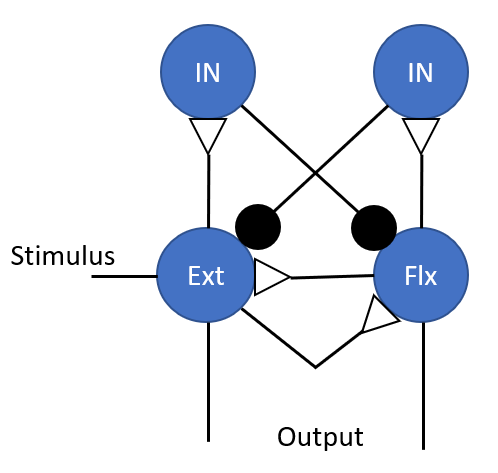
\includegraphics[width=\linewidth,height=0.20\textheight,keepaspectratio]{RGnetwork.PNG}
\end{minipage}\hfill
\begin{minipage}[t]{0.47\textwidth}\centering
\textbf{(B) Pattern formation}\par\smallskip
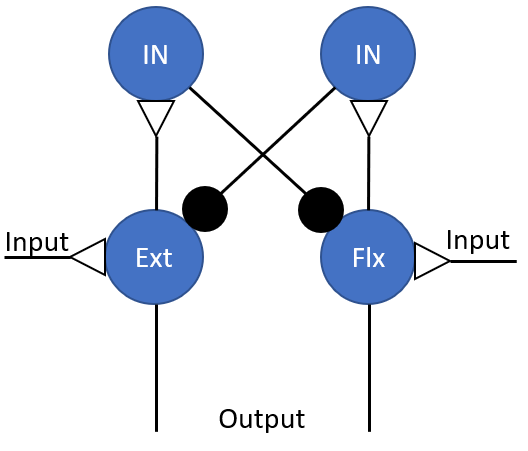
\includegraphics[width=\linewidth,height=0.20\textheight,keepaspectratio]{PFnetwork.PNG}
\end{minipage}
\par\medskip
\textbf{(C) Sensorimotor organization}\par\smallskip
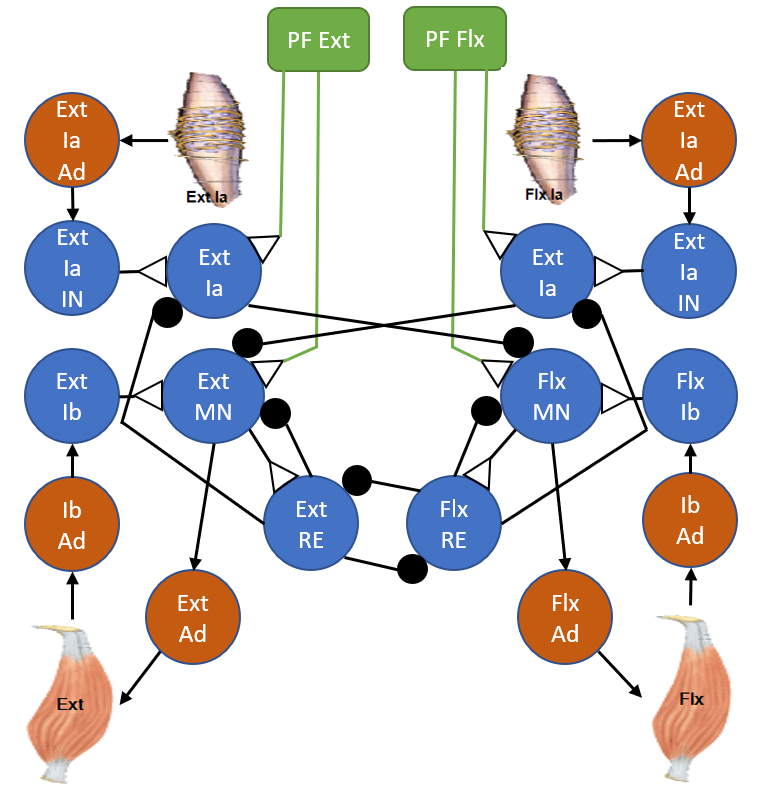
\includegraphics[width=0.76\textwidth,height=0.39\textheight,keepaspectratio]{sensoryMotor_Network.PNG}
\caption[AnimatLab controller reference schematics]{Archived AnimatLab motifs: rhythm generation (A), pattern formation (B), and sensorimotor organization (C). Ext and Flx denote antagonist pathways; IN denotes interneurons, MN motor neurons, and Ia and Ib muscle afferents. Triangles and circles distinguish excitatory and inhibitory connections.}
\label{fig:animatlab_controller_motifs}
\end{figure}

A \qty{10}{\second} instrumented run recorded joint, neural, sensory, and body-motion channels at a \qty{0.2}{\milli\second} interval. Contact-sensory recordings are membrane voltages, not contact forces. The initial external horizontal force and the limited window prevent the joint traces from establishing stable walking.

\begin{figure}[htbp]
\centering
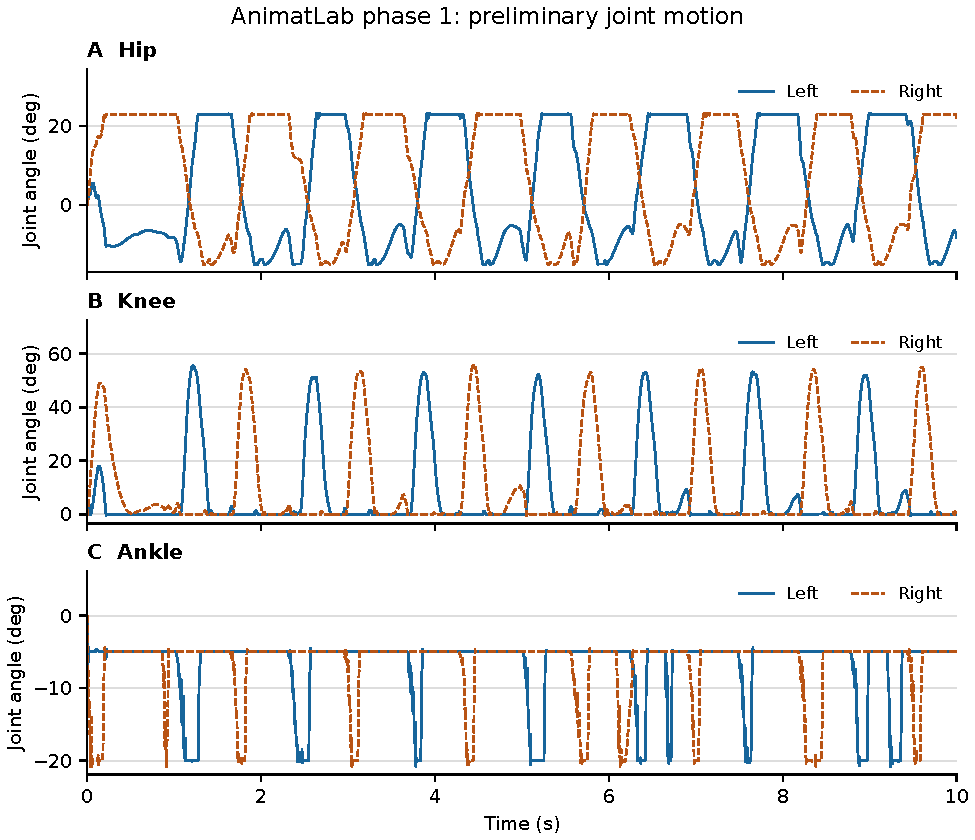
\includegraphics[width=\textwidth,height=0.60\textheight,keepaspectratio]{animatlab_phase1_joint_angles.pdf}
\caption[AnimatLab phase-1 hip, knee, and ankle recordings]{Bilateral hip (A), knee (B), and ankle (C) angles in the recorded joint conventions. All 50,001 samples in the \qty{10}{\second} window are retained. An external horizontal force acts during the first second. The recordings show motion, not validated walking or ground-contact gating.}
\label{fig:animatlab_phase1_preliminary}
\end{figure}

\begin{figure}[p]
\centering
\begin{minipage}[t]{0.48\textwidth}\centering
\textbf{(A) Converted robot}\par\smallskip
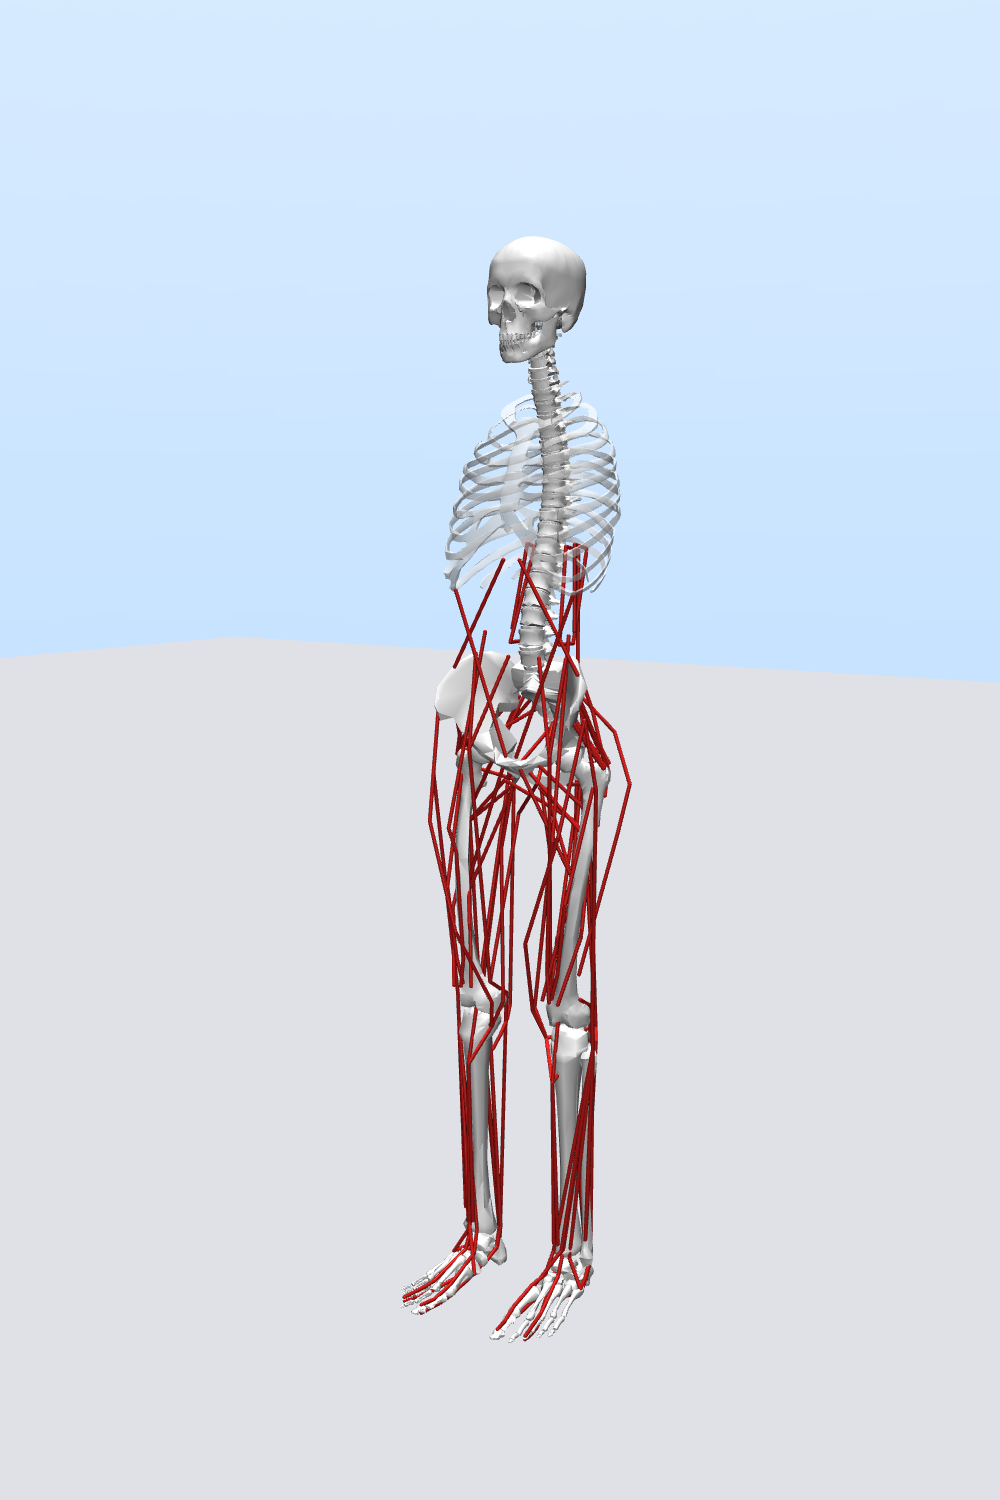
\includegraphics[width=\linewidth,height=0.53\textheight,keepaspectratio]{mujoco_converted_robot.png}
\end{minipage}\hfill
\begin{minipage}[t]{0.48\textwidth}\centering
\textbf{(B) SNS-Simscape knee model}\par\smallskip
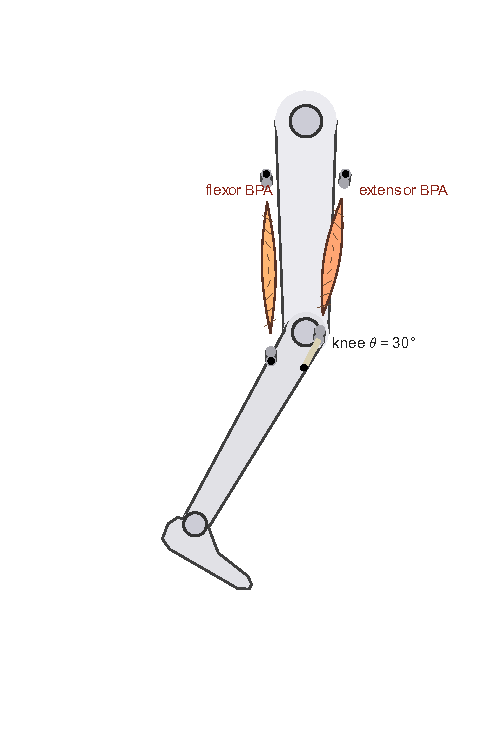
\includegraphics[width=\linewidth,height=0.53\textheight,keepaspectratio]{knee_model_current.pdf}
\end{minipage}
\caption[Mechanical model representations]{Converted Gait2392 robot (A) and the antagonist-BPA knee illustration used in the current SNS-Simscape demonstration (B). The two panels represent different models; scales differ.}
\label{fig:mujoco_model_views}
\end{figure}

\section{Controller Ports and Reference Checks}\label{sec:sns_ports}\label{sec:crossengine_methods}

The matched W2L test compares implementations from a common circuit specification under identical drive and contact inputs, using burst period, bilateral phase, burst count, and voltage correlation. The Deng controller port was checked separately: a current-pulse test produced a \qty{1.938}{\second} period against a \qty{1.94}{\second} NumPy reference, with antagonist correlation $r=-0.86$. Agreement on these tests does not establish long-term phase agreement in every network.

The Deng port comparison above establishes agreement between the translated implementations, not quantitative reproduction of the original AnimatLab model. A separate rerun of the archived original produced a period of approximately \qty{0.221}{\second}, compared with \qty{1.938}{\second} in the translated test. Antagonist alternation was present, but the bilateral rhythm was in phase. The original and translated models use different parameterizations, so these results do not establish quantitative reproduction of the original dynamics. Their rhythm-generator perturbation responses do agree qualitatively: activity is perturbed and then recovers without sustained suppression. An earlier suppression interpretation arose from counting no peaks inside a window that also contained no baseline peaks; comparing the perturbed and unperturbed sequences resolves that analysis error.

The full exported network agreed with its NumPy reference to \qty{4.2e-06}{\milli\volt} over the early transient across 410 neurons. Its subsequent divergence and the tonic-drive fixed-point discrepancy reported in Chapter~\ref{ch:sns} limit parameter transfer. The OpenSim-derived Simscape mechanism contains 1,446 blocks and 149 joints; mechanism compilation is distinct from completing its neural and muscle coupling.

\subsection{Transient Knee Sensory-Current Response}\label{sec:app_knee_transient}

The knee block model was tested from a settled operating point using a rectangular current pulse added after the spindle transducer and before the extensor Ia sensory-neuron membrane input. Stimulus and no-stimulus cases start from the same initial conditions and run continuously for \qty{50}{\second}; the \qty{2}{\nano\ampere} pulse acts from 30.000 to \qty{30.030}{\second}. The original configuration did not settle: its knee angle spanned \ang{0.712} during the 25--30 s baseline window. Its former startup comparison is therefore not used to demonstrate transient reflex recovery.

The graded-response comparison changes exactly six parameters: the two MN output ramp widths from 1 to \qty{10}{\milli\volt}, and the four Ia synaptic ramp widths from 0.5 to \qty{10}{\milli\volt}. Equations, thresholds, conductances, wiring, mechanics, tonic drives, and activation dynamics are retained. This reduces loop gain as an explicit engineering comparison, rather than fitting physiological parameters. The simple actuator-force law is distinct from the characterized BPA model of Chapter~\ref{ch:muscles}. The flexor activation is zero at baseline, so the experiment does not establish suppression of a tonically active antagonist.

The modified configuration passes baseline settling tests for angle, velocity, all six membrane states, and both activations. Its paper-coordinate baseline is \ang{-42.6392}; positive excursions indicate extension. Extension peaks at \ang{1.0908} after \qty{111}{\milli\second}. Recovery requires displacement within \ang{0.01} of baseline and absolute angular velocity below \qty{1e-4}{\radian\per\second}; both remain within those bounds from \qty{6.355}{\second} after stimulus onset. The late residual is approximately \ang{9.3e-7}. A fresh-process replay reproduces the resampled pulse arrays exactly. Halving the ODE45 maximum step from 1 to \qty{0.5}{\milli\second}, at unchanged tolerances, changes the angle trace by at most \ang{5.21e-5}. Comparisons use linear interpolation onto a 1 ms grid, without smoothing. These checks establish numerical recovery in the model, not physiological reflex fidelity.

\begin{figure}[p]
\centering
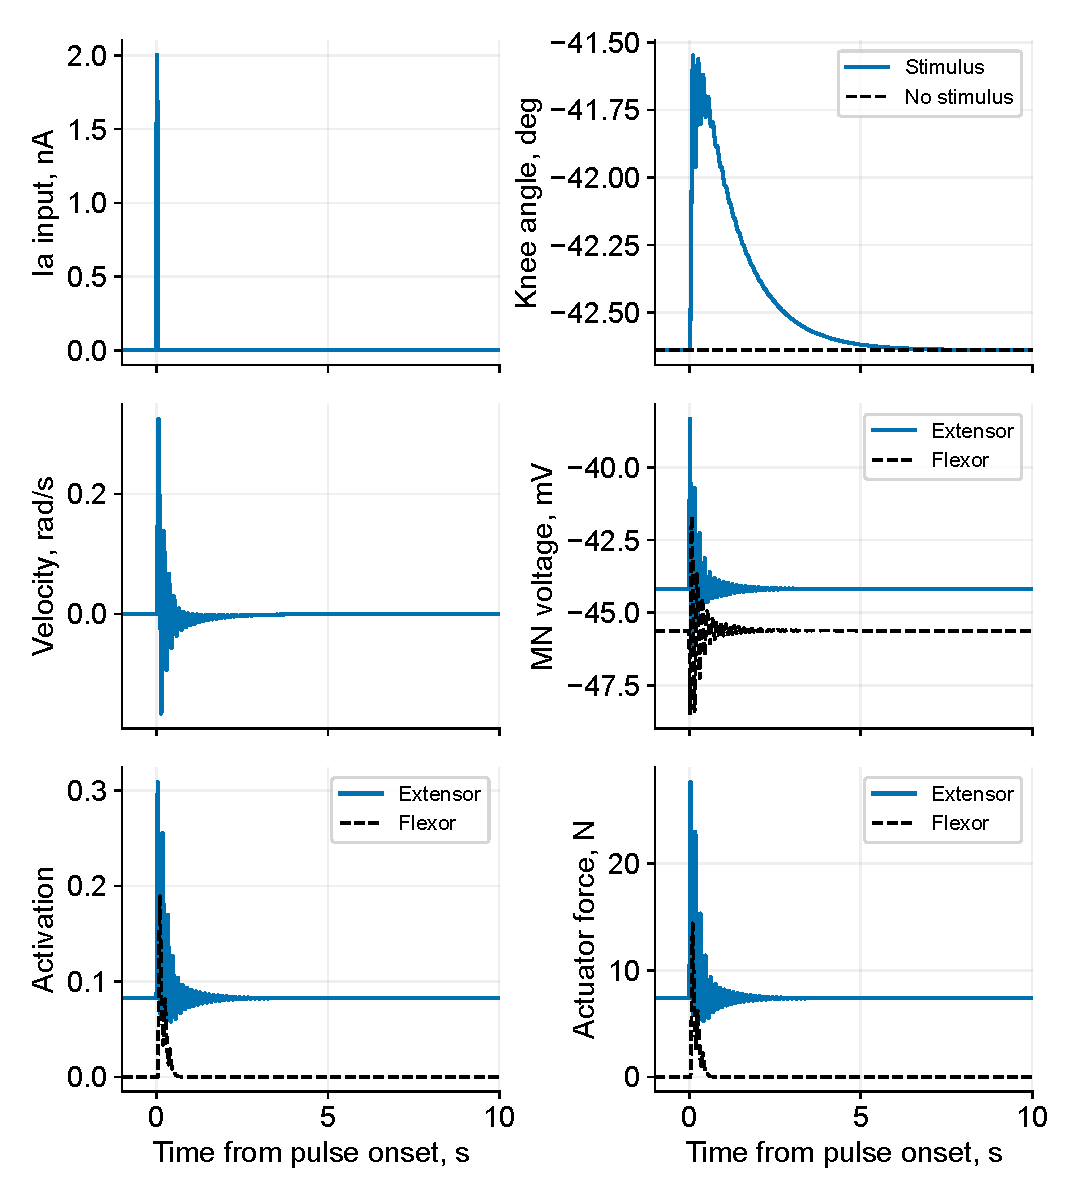
\includegraphics[width=\textwidth,height=0.76\textheight,keepaspectratio]{knee_transient_response.pdf}
\caption[Transient knee sensory-current test]{Stimulus, knee angle, angular velocity, MN voltages, activations, and actuator forces in the graded-response knee model. The pulse enters the extensor Ia sensory neuron after settling. Knee angle is compared with the no-stimulus control; extensor and flexor signals are distinguished in the other paired panels. The display applies only the sign conversion to flexion-negative coordinates.}
\label{fig:app_knee_transient}
\end{figure}

\subsection{A Published Neural Mechanism as a Verification Target}\label{sec:rybak_verification}

The reduced Python implementation of the two-level circuit of \citet{rybak_modelling_2006} passed 13 checks covering drive-dependent activity, repeatability, and the distinction between resetting and non-resetting deletions. Stimulating the pattern-formation extensor population suppressed flexor motor output while the rhythm generator continued, so flexor activity resumed at its expected phase. Stimulating the rhythm-generator extensor population also suppressed flexor output but shifted the subsequent rhythm phase. This comparison tests the functional separation between rhythm generation and pattern formation: similar missing motor bursts can arise through different neural mechanisms. It is a neural-only verification of the translated circuit, independent of a mechanical model and separate from the Simulink demonstrations.

\subsection{RG, PF, and MN Stimulus Tests}\label{sec:app_layer_stimulus}

The fourteen-neuron Deng-derived implementation follows the circuit used in SNS-Toolbox demonstrations \citep{deng_neuromechanical_2019,nourse_sns_2023}. A \qty{0.1}{\milli\second} Euler step reproduced the existing neural integrator's complete 24-second baseline voltage trace exactly in the tested process. The baseline period was \qty{1.938}{\second}. Neural output drove the existing suspended, unilateral W2L mechanical model without afferent return. Hip commands came from the MN outputs; knee and ankle commands used the existing PF-to-activation mapping. This configuration tests transmitted circuit effects, not the original rat mechanics or bilateral walking.

The initial sweep applied $+2$ and $+10$ nA to each layer for 0.1 and 0.5 seconds, together with two direct MN inhibitory controls. None met the deletion criterion. Subsequent stronger-current control series, including stimuli lasting two baseline periods (\qty{3.876}{\second}), retained the same circuit and mechanical parameters (Table~\ref{tab:layer_stimulus}). RG and PF stimuli began one-quarter cycle after a baseline RG onset; MN inhibition began 0.05 seconds into a baseline motor burst. Positive currents target the extensor RG or hip-PF population; negative currents target the hip-flexor MN. These currents are mechanistic controls, not experimentally calibrated physiological stimuli.

A deletion required at least \qty{20}{\milli\second} of baseline motor activity in the stimulus window and suppression of at least half of that activity, using an activation threshold of 0.5. Phase residuals compare the final four recovered onsets with the nearest baseline onset, normalized by the baseline period. Residuals at or below 0.05 cycles were classified as non-resetting, and those at or above 0.15 as shifted; intermediate values remained indeterminate. RG and motor residuals were assessed separately. The two-cycle stimuli suppressed both expected flexor burst onsets at all three layers. Baseline and stimulated neural and mechanical trajectories were identical before stimulus onset. The one-second PF pulse shifted the motor pattern without resetting the RG clock, whereas the two-cycle PF pulse preserved both schedules. The duration dependence cautions against treating every motor phase shift as an RG reset.

\begin{table}[htbp]
\centering\small
\caption[Layer-specific stimulation controls]{Stronger-current controls in the reduced Deng-derived circuit. Phase residuals are fractions of the baseline cycle. ``No deletion'' means the specified suppression criterion was not met.}
\label{tab:layer_stimulus}
\begin{tabularx}{\textwidth}{@{}lrrcc>{\raggedright\arraybackslash}X@{}}
\toprule
Target & nA & s & RG phase & MN phase & Outcome \\
\midrule
RG & $+50$ & 0.5 & 0.052 & 0.052 & Brief suppression; phase indeterminate \\
RG & $+50$ & 1.0 & 0.307 & 0.307 & Suppression; RG and MN shifted \\
PF & $+50$ & 0.5 & 0.000 & 0.000 & Brief suppression; schedule preserved \\
PF & $+50$ & 1.0 & 0.000 & 0.208 & Motor pattern shifted; RG preserved \\
MN & $-100$ & 0.5 & 0.000 & 0.000 & No deletion \\
MN & $-500$ & 0.5 & 0.000 & 0.000 & Brief suppression; schedule preserved \\
RG & $+50$ & 3.876 & 0.211 & 0.211 & Resetting deletion \\
PF & $+50$ & 3.876 & 0.000 & 0.000 & Non-resetting deletion \\
MN & $-500$ & 3.876 & 0.000 & 0.000 & Non-resetting deletion \\
\bottomrule
\end{tabularx}
\end{table}

\begin{figure}[p]
\centering
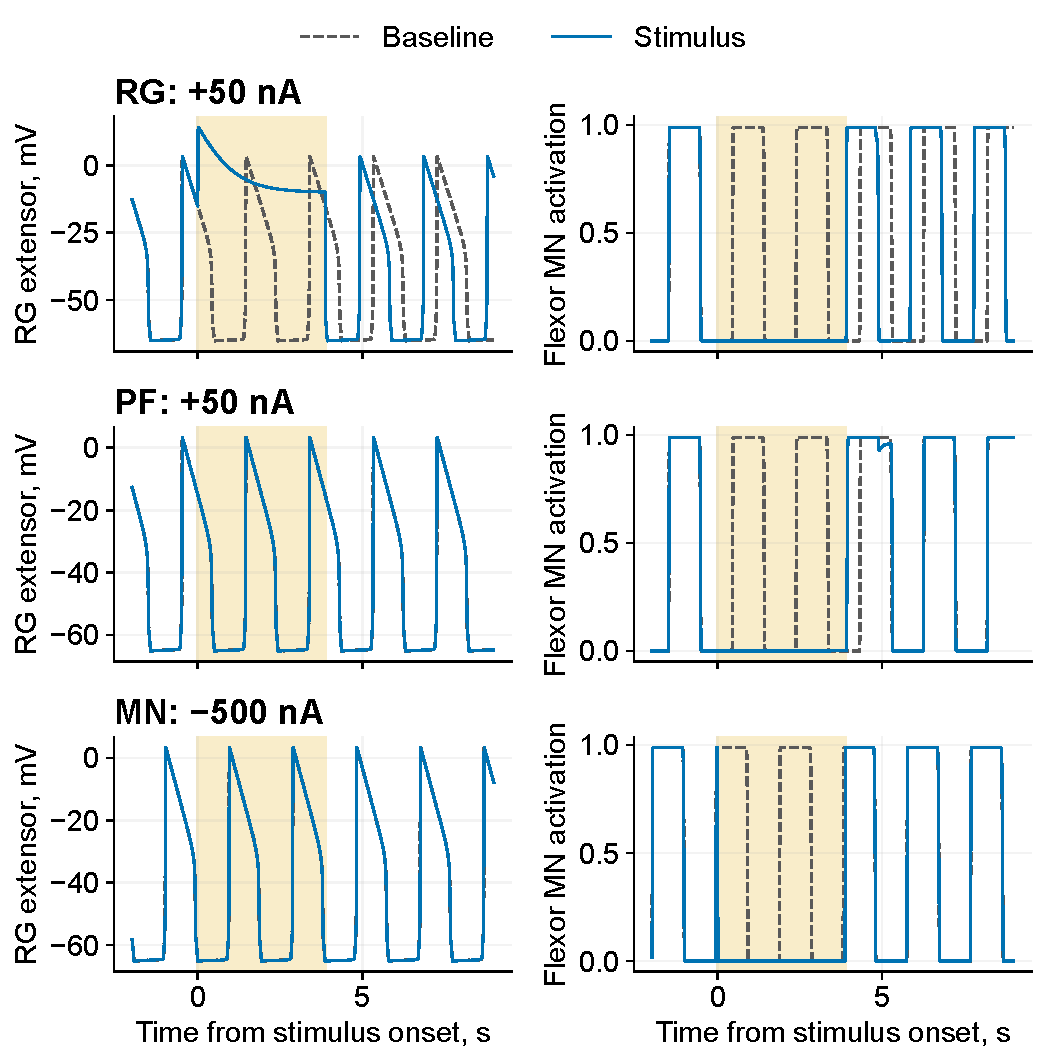
\includegraphics[width=\textwidth,height=0.74\textheight,keepaspectratio]{layer_stimulus_validation.pdf}
\caption[Layer-specific stimuli and downstream responses]{Matched baseline and stimulus responses in the reduced Deng-derived circuit coupled to a suspended model. All stimuli last two baseline periods. Rows show RG stimulation, PF stimulation, and direct flexor-MN inhibition; columns show RG voltage and flexor-MN activation. Shading marks the applied stimulus. The RG intervention shifts subsequent timing, whereas the displayed PF and MN interventions preserve the RG schedule.}
\label{fig:layer_stimulus_validation}
\end{figure}

\FloatBarrier

\subsection{Archived AnimatLab Models}\label{sec:animatlab_validation}

Headless reruns tested whether archived models reproduced their reference behavior in the original simulator. Eleven targetable rhythm and gait metrics passed their acceptance bands. The bilateral contact-driven model's rhythm generators had periods of \qty{0.450}{} and \qty{0.467}{\second}; the modern W2L model showed joint oscillations at \qty{2.25}{\Hz}. The Li-model rerun reached \qty{0.637}{\meter\per\second} with step periods near \qty{1.3}{\second} \citep{li_bipedal_2017}. These are reference-model checks, not results for the combined Deng--Li model or evidence of unsupported walking.

A separate MuJoCo translation of the Li controller and body did not reproduce that original-simulator walking result. In a 20-second ground test, mean forward speed was \qty{0.040}{\meter\per\second}, with eleven detected right-foot stance episodes and none on the left. The right-side period of \qty{1.294}{\second} alone therefore did not establish bilateral stepping. This failure distinguishes reproduction of the source model from successful transfer to another simulator.

\section{Tuning and Supported Evaluations}\label{sec:sns_tuning_methods}\label{sec:sns_curriculum}

Free network gains were searched with a tree-structured Parzen estimator, with each candidate evaluated through simulation. The staged procedure separates suspended rhythm generation, sensory feedback, standing, and ground evaluations (Table~\ref{tab:sns_curriculum}). Finalists were checked under \qty{1}{\percent} multiplicative parameter perturbations and changes in drive. Such checks probe the neighborhood of a selected configuration; they do not establish robustness to untested loads or removal of the harness.

The cycle-shape metric assigns zero to perfect agreement. A run without detectable cycles returns $-25$ as a reserved failure value. Because this value is numerically greater than the genuine-gait scores below, failed runs must be identified before ranking scores. That value itself is not a valid measure of gait quality.

The curriculum is shown in Table~\ref{tab:sns_curriculum} in Chapter~\ref{ch:sns}.

\subsection{Reference-Library Comparison}\label{sec:gait_library_results}

The 43-cycle library contains 32 running trials from eight subjects at four speeds, ten walking references, and a predicted-walking cycle. The walking references span prescribed speeds of \qtyrange{0.5}{2.0}{\meter\per\second} and self-selected trials. The production network (\texttt{s3k}), reduced-connection network (\texttt{s3kpruned}), six-group activation network (\texttt{syn6}), and W2L-organization network (\texttt{w2lvar}) were scored without treating a good tuning-reference score as evidence of generalization. Library scores were substantially more negative (Table~\ref{tab:gait_sweep}), and the evaluations showed unilateral or asymmetric gait. This comparison bounds transfer to the available references; it does not validate normal human walking.

Table~\ref{tab:gait_sweep} uses the production pipeline's cycle-shape kinematic score. The tuning-reference column reports each configuration on its tuning reference; the library mean averages that score over all 43 reference cycles.

\begin{table}[htbp]
\caption{Four controller configurations evaluated on their tuning reference and the 43-cycle reference library. For genuine gait cycles, larger kinematic scores indicate closer agreement; zero is perfect agreement.}
\label{tab:gait_sweep}
\begin{tabular}{@{}lrrl@{}}
\toprule
 & \textbf{Tuning-ref.} & \textbf{Library mean} & \textbf{Most negative reference} \\
 & \textbf{score} & \textbf{score (43 refs)} & \textbf{(score)} \\
\midrule
\texttt{s3k}        & $-186.4$ & $-8776$ & \texttt{Case\_40\_motion} ($-8841$) \\
\texttt{s3kpruned}  & $-176.1$ & $-6924$ & \texttt{Case\_40\_motion} ($-6986$) \\
\texttt{syn6}       & $-200.4$ & $-9961$ & \texttt{Case\_40\_motion} ($-10040$) \\
\texttt{w2lvar}     & $-144.5$ & $-5808$ & \texttt{subject08\_Run\_20002} ($-5896$) \\
\bottomrule
\end{tabular}
\end{table}

\subsection{Direct Kinematics Overlay}\label{sec:app_ik_overlay}

The saved human-model controller reproduced its cycle-shape score of $-145.07$ in an independent process. The direct overlay in Figure~\ref{fig:gait2392_ik_overlay} uses the Gait2392 walking inverse-kinematics trajectory and its paired ground-reaction-force file. Model cycles begin when vertical foot loading crosses \qty{50}{\newton}; reference stance is defined using the same force threshold. Ten cycles per side, with durations between 0.35 and 2.5 seconds, were retained using the existing cycle detector. Each leg was aligned to its own onset and resampled over the gait cycle, without fitting phase, subtracting the mean angle, or scaling amplitude.

Mean cycle periods were \qty{1.285}{\second} on the right and \qty{1.254}{\second} on the left, compared with \qty{1.233}{\second} and \qty{1.213}{\second} in the reference. Model stance fractions were 0.710 and 0.649, compared with 0.610 in the reference. Table~\ref{tab:ik_absolute_rmse} reports absolute-angle errors between mean cycles. These errors retain posture offsets and are distinct from the mean-removed cycle-shape errors used in tuning. The hip and knee mismatches show why cycle counts and a scalar score must be accompanied by the trajectories and contact timing.

\begin{table}[htbp]
\centering
\caption[Absolute-angle errors against Gait2392 inverse kinematics]{Unshifted absolute-angle RMSE between mean model and reference cycles, in degrees.}
\label{tab:ik_absolute_rmse}
\begin{tabular}{lrr}
\toprule
Joint & Right & Left \\
\midrule
Hip & 28.03 & 24.65 \\
Knee & 27.44 & 28.45 \\
Ankle & 8.71 & 7.38 \\
\bottomrule
\end{tabular}
\end{table}

\subsection{Pathway-Removal Tests}\label{sec:walker_variant_results}

Individual pathway classes were removed from each selected configuration and the model re-evaluated on its tuning reference (Table~\ref{tab:walker_ablations}). Removing Ia feedback from the production configuration eliminated detected cycles. Other removals changed the score without necessarily eliminating movement. The different response of the six-synergy variant shows that these dependencies belong to the tested network configurations, rather than constituting a general claim about biological necessity. The systematic pattern-formation and motoneuron stimulation series for these full Gait2392 networks was not completed. The reduced-circuit tests in Section~\ref{sec:app_layer_stimulus} address a separate, smaller model.

\begin{table}[htbp]
\caption{Pathway-removal tests on the tuning reference. Full-model rows give unchanged baselines. A score of $-25$ is the fixed no-cycle fallback and denotes failure, despite exceeding the genuine-gait scores.}
\label{tab:walker_ablations}
\small\begin{tabularx}{\textwidth}{@{}>{\raggedright\arraybackslash}p{0.20\textwidth}>{\raggedright\arraybackslash}X>{\raggedright\arraybackslash}p{0.24\textwidth}@{}}
\toprule
\textbf{Configuration} & \textbf{Removed pathway} & \textbf{Score} \\
\midrule
\texttt{s3k} (full model) & none & $-186.4$ \\
 & Ia afferents & $-25$ (no cycles detected) \\
 & all afferent classes & $-267.8$ \\
 & Renshaw cells & $-267.3$ \\
 & group-II afferents & $-255.2$ \\
 & Ib afferents & $-180.3$ \\
 & contact channels & $-183.9$ \\
 & interleg commissural pathways & $-174.9$ \\
\addlinespace
\texttt{syn6} (full model) & none & $-200.4$ \\
 & all afferent classes & $-190.5$ \\
\addlinespace
\texttt{w2lvar} (full model) & none & $-144.5$ \\
 & Ia afferents & $-273.5$ \\
 & weak rhythm-generator mutual excitation & $-279.9$ \\
 & Renshaw cells & $-142.4$ \\
\bottomrule
\end{tabularx}
\end{table}

\section{Spiking-Neuron Comparisons}\label{sec:spiking_methods}\label{sec:spiking_results}\label{sec:disc_spiking}

The spiking variants replace afferent, rhythm-generator, and interneuron populations while retaining graded motor neurons. Synapses onto motor neurons are calibrated by mean conductance, preserving the continuous activation interface. This construction does not require the network dynamics or resulting movement to remain unchanged. Calibration and full conversion tables are in Appendix~\ref{app:neuron_equations}.

\subsection{MuJoCo Network and Ground Evaluation}

Under constant drive, the non-spiking and spiking rhythm periods were \qty{0.399}{} and \qty{0.621}{\second}, respectively (Figure~\ref{fig:spike_rhythm}). The spiking period is \qty{55.6}{\percent} longer. Timing agreement therefore requires more than copying the selected parameters. The untuned spiking variant produced bilateral cycling in a ground evaluation where the non-spiking winner cycled predominantly on one side (Table~\ref{tab:spike_ground}; Figure~\ref{fig:spike_ground}). This individual comparison motivates further controlled testing; it does not establish superiority of spiking control.

\begin{figure}[htbp]
\centering
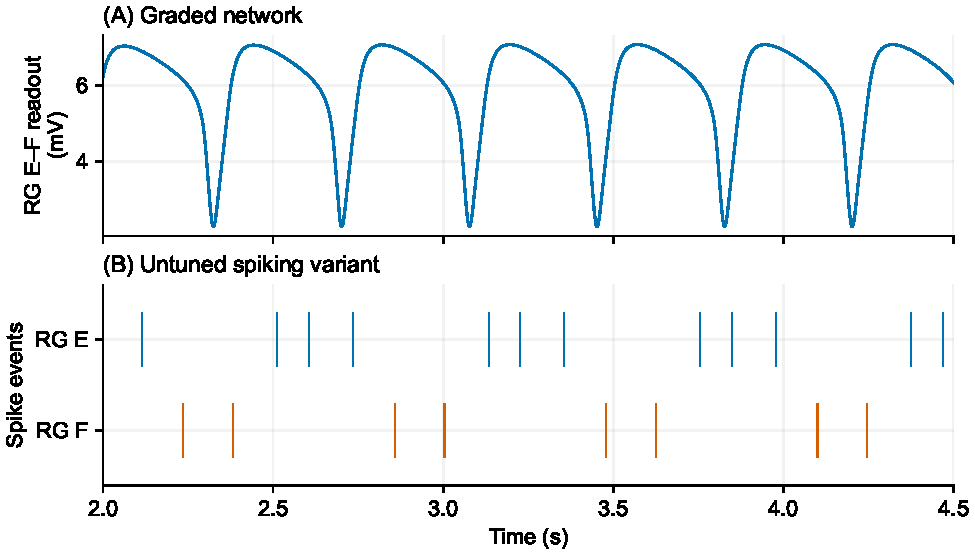
\includegraphics[width=\textwidth]{spiking_mirror_rhythm.pdf}
% ALT TEXT: see spiking_mirror_rhythm_alt.txt beside the figure file.
\caption[Constant-drive rhythm, non-spiking versus spiking]{Constant-drive rhythm in the non-spiking network (A) and spiking variant (B). The observed periods are \qty{0.399}{} and \qty{0.621}{\second}; the latter is \qty{55.6}{\percent} longer. The panels use different neural readouts: graded population difference versus individual spiking cells.}
\label{fig:spike_rhythm}
\end{figure}

\begin{table}[htbp]
\caption{Supported ground evaluation at the same selected parameters (16 s), with no spiking re-tuning. Knee minima and contact duty are computed over detected cycles. The kinematic score is a cycle-shape error metric: zero denotes perfect agreement, and less negative scores indicate closer agreement.}
\label{tab:spike_ground}
\begin{tabular}{@{}lcc@{}}
\toprule
\textbf{Metric} & \textbf{Non-spiking winner} & \textbf{Spiking mirror (untuned)} \\
\midrule
Kinematic score                & $-161.57$          & $-236.35$ \\
Gait cycles, right / left      & 9 / 0 (left frozen) & 8 / 9 (bilateral) \\
Cycle knee minimum             & \ang{-64.3}         & \ang{-79.8} \\
Contact duty, right / left     & 0.637 / 0.985       & 0.799 / 0.856 \\
Maximum pelvis tilt            & \ang{22.1}          & \ang{19.2} \\
Non-finite states / fell       & no / up             & no / up \\
\bottomrule
\end{tabular}
\end{table}

\begin{figure}[htbp]
\centering
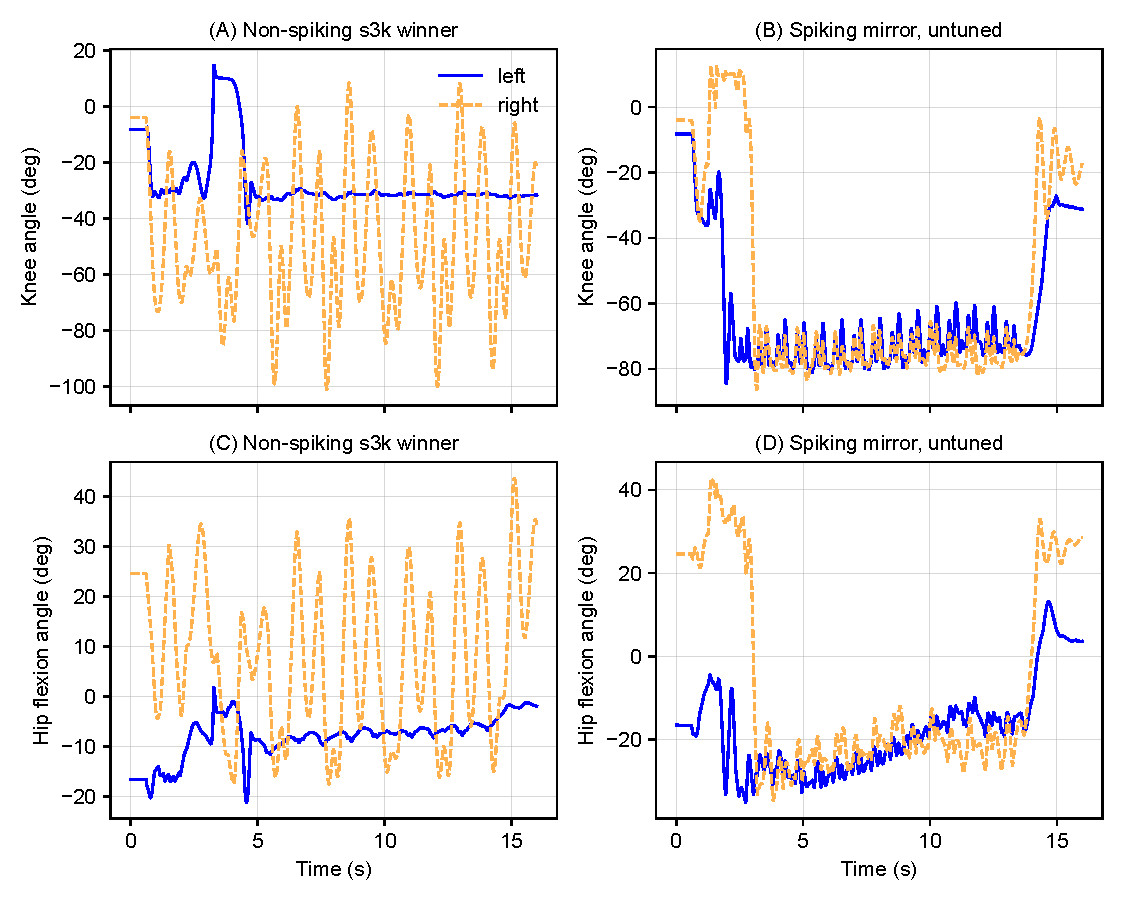
\includegraphics[width=\textwidth]{spiking_mirror_ground_gait.pdf}
% ALT TEXT: see spiking_mirror_ground_gait_alt.txt beside the figure file.
\caption[Ground gait, non-spiking winner versus untuned spiking mirror]{Ground-evaluation joint angles at the non-spiking winner parameters. The non-spiking model cycles predominantly on the right (A, C), while the untuned spiking variant cycles both legs (B, D). Solid indigo denotes left, and dashed orange right. Both use the supported evaluation protocol.}
\label{fig:spike_ground}
\end{figure}

\subsection{Simulink Demonstrations}

The graded and spiking knee-reflex demonstrations were compared over matched \qty{5}{\second} runs (Table~\ref{tab:spike_knee}; Figure~\ref{fig:spike_knee}). The beverage example retained approximately the same sag, \ang{2.02} versus \ang{2.00}, compared with \ang{7.85} without the reflex. These examples demonstrate transfer of particular reflex responses after calibration, not invariance of all controlled behavior to neural coding.

\begin{table}[htbp]
\caption{Knee-reflex demonstration, graded baseline versus spiking twin at the matched operating point (5 s runs; settle statistics over the last \qty{2}{\second}).}
\label{tab:spike_knee}
\small\begin{tabularx}{\textwidth}{@{}>{\raggedright\arraybackslash}p{0.42\textwidth}>{\raggedright\arraybackslash}X>{\raggedright\arraybackslash}X@{}}
\toprule
\textbf{Metric} & \textbf{Baseline} & \textbf{Spiking twin} \\
\midrule
Knee angle at \qty{0.05}{\second}   & \ang{15.79} & \ang{15.79} \\
Settle mean (last \qty{2}{\second}) & \ang{43.5}  & \ang{44.4} \\
Settle range                        & \ang{41.6}--\ang{44.9} & \ang{41.9}--\ang{46.7} \\
Extensor / flexor activation (window means) & 0.53 / 0.53 & 0.58 / 0.56 \\
Antagonist alternation              & \qty{0.5}{\hertz}--\qty{2}{\hertz} & \qty{7.4}{\hertz} (dominant peak) \\
Ia interneuron firing at settle     & graded, subthreshold & \qty{95}{\hertz}; Ib \qty{0}{\hertz} \\
\bottomrule
\end{tabularx}
\end{table}

\begin{figure}[htbp]
\centering
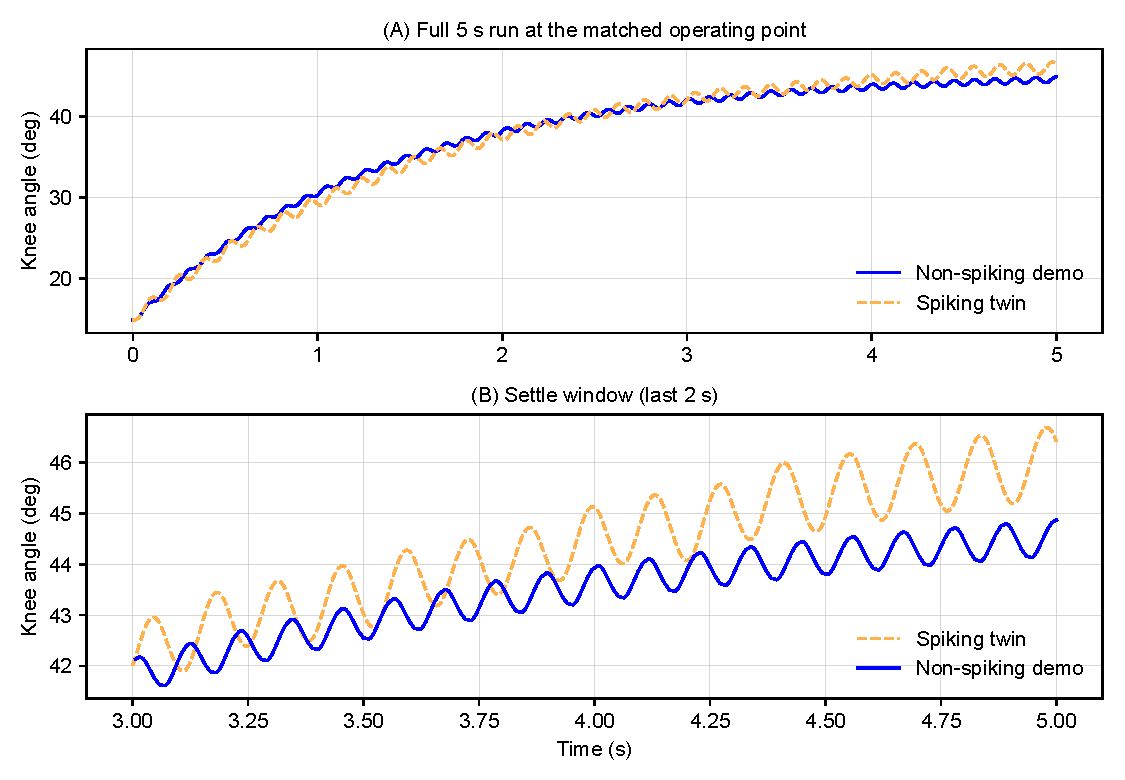
\includegraphics[width=\textwidth]{simulink_knee_spiking_twin.pdf}
% ALT TEXT: see simulink_knee_spiking_twin_alt.txt beside the figure file.
\caption[Simulink knee-reflex twin, baseline versus spiking]{Knee-reflex demonstration at the matched operating point: graded baseline (solid indigo) and spiking variant (dashed orange). Full \qty{5}{\second} run (A) and final \qty{2}{\second} window (B). The spiking response has a slightly wider oscillation band.}
\label{fig:spike_knee}
\end{figure}

\subsection{AnimatLab Conversions}

The tested spiking conversions did not preserve the graded models' rhythm (Table~\ref{tab:spike_animatlab}). Converting thresholds while retaining graded synapses preserved near-baseline oscillations, whereas converting synaptic amplitudes and decay changed or eliminated alternation. These results identify the synapse conversion as a limitation of this mapping. They do not demonstrate that a suitably calibrated spiking implementation cannot reproduce the reference behavior.

\begin{table}[htbp]
\caption{AnimatLab spiking conversions versus their graded baselines (5.1 s headless runs; joint ranges in degrees where the rhythm survives). The thresholds-only ablation converts the neurons but keeps the graded synapses.}
\label{tab:spike_animatlab}
\small
\begin{tabular}{@{}lcc@{}}
\toprule
\textbf{Variant} & \textbf{Baseline (graded)} & \textbf{Spiking copy} \\
\midrule
Two-layer walker     & \qty{0.443}{\second} rhythm;   & dead (2 spikes; \\
                     & hip $-15$ to $+23$, knee $-1$ to $+60$ & hip pinned near $+6$) \\
Bilateral variant    & \qty{0.462}{\second}; antiphase $-0.42$ cycle & latched; one side at \qty{442}{\hertz}--\qty{450}{\hertz} \\
Reorganized project  & latched (tonic drives) & synchronous \qty{11.8}{\hertz} co-bursting; \\
(standalone export)  &                        & same-leg envelopes $r = 1.000$ at lag 0 \\
Thresholds only      & \multirow{2}{*}{hip $-15$ to $+23$, knee $-1$ to $+60$} & oscillates: hip $-15.1$ to $+23.2$, \\
(graded synapses)    &                        & knee $-0.8$ to $+47.9$ \\
\bottomrule
\end{tabular}
\end{table}

\section{Supported BPA-Robot Evaluations}\label{sec:sns_controller_comparison}

The BPA-actuated walker exercised the chain from neural activation through the actuator force model to multi-joint motion. In the supported air-stepping run, the virtual harness carried \qty{70}{\percent} of the \qty{411}{\newton} body weight. The period was \qty{1.542}{\second}, knee RoM was \ang{63.5}, and peak forces were \qty{880}{} and \qty{1372}{\newton}, at a peak pressure of \qty{372}{\kPa}. 

With split left/right drives and retuned feedback, the W2L robot progressed \qty{1.72}{\meter} over \qty{30}{\second} under the support protocol. It retained progression at \qty{60}{\percent} drive and passed 12 of 12 perturbed reruns, but did not satisfy the strict contact-duty walking criterion; below that drive the gait ceased. The mechanical support was not weaned.

In the separate human-model drive-weaning study, the selected score improved from $-161.57$ to $-145.07$, with ten contact cycles per leg and contact duties of 0.71 and 0.65. It passed eight of eight perturbed reruns and retained bilateral stepping down to zero hand drive. The motion remained in place under support. These two studies distinguish reduced neural assistance from reduced mechanical assistance.



\subsection{Independent Replays and Remaining Mechanical Assistance}\label{sec:app_supported_replays}

A separate W2L configuration was evaluated after correcting the delivery of saved per-target gains to the evaluator. Four independent \qty{30}{\second} replays produced identical trajectories. Over the \qtyrange{4.5}{30}{\second} analysis window, the run had 28 left and 21 right contact events, a median bilateral phase of 0.496 cycles, forward displacement of \qty{2.246}{\meter}, and fitted speed of \qty{0.0918}{\meter\per\second}. All twelve independent reruns with \qty{1}{\percent} parameter perturbations passed the supported-stepping criterion. These are results for this configuration, distinct from the drive-weaning study above.

Removing nominal constant weight support did not remove the position-control harness: its mean vertical force still supplied approximately \qty{16.76}{\percent} of body weight. Contact duty remained below the strict walking criterion. Thus, repeatable supported stepping was demonstrated, while harness-free walking was not. An accelerated neural backend preserved the complete reference trajectories and reduced the isolated neural-step cost by a factor of 1.425; this does not establish the same speed improvement for the complete neuromechanical simulation.

\subsection{Pathway Deletions and Stimulus Tests}\label{sec:app_w2l_perturbations}

The recovered W2L configuration was evaluated with nominal weight support set to 0.25 and the remaining controller settings fixed. Mild and strong drive reductions, forward and backward \qty{40}{\newton} pushes, and separate Ia, Ib, Renshaw, crossed-heel, and heel-cascade deletions retained the supported-stepping criterion. Their effects differed: Renshaw deletion reduced forward displacement to \qty{0.081}{\meter}, while commissural deletion failed bilateral stepping. Disabling all sensory feedback retained joint cycling and \qty{1.996}{\meter} progression but shifted median contact phase to 0.223 cycles, outside the accepted alternation range. The intact comparison produced \qty{2.239}{\meter} and a phase of 0.498 cycles. These experiments distinguish rhythm generation, progression, and bilateral contact coordination, rather than treating them as interchangeable outcomes.

\begin{figure}[htbp]
\centering
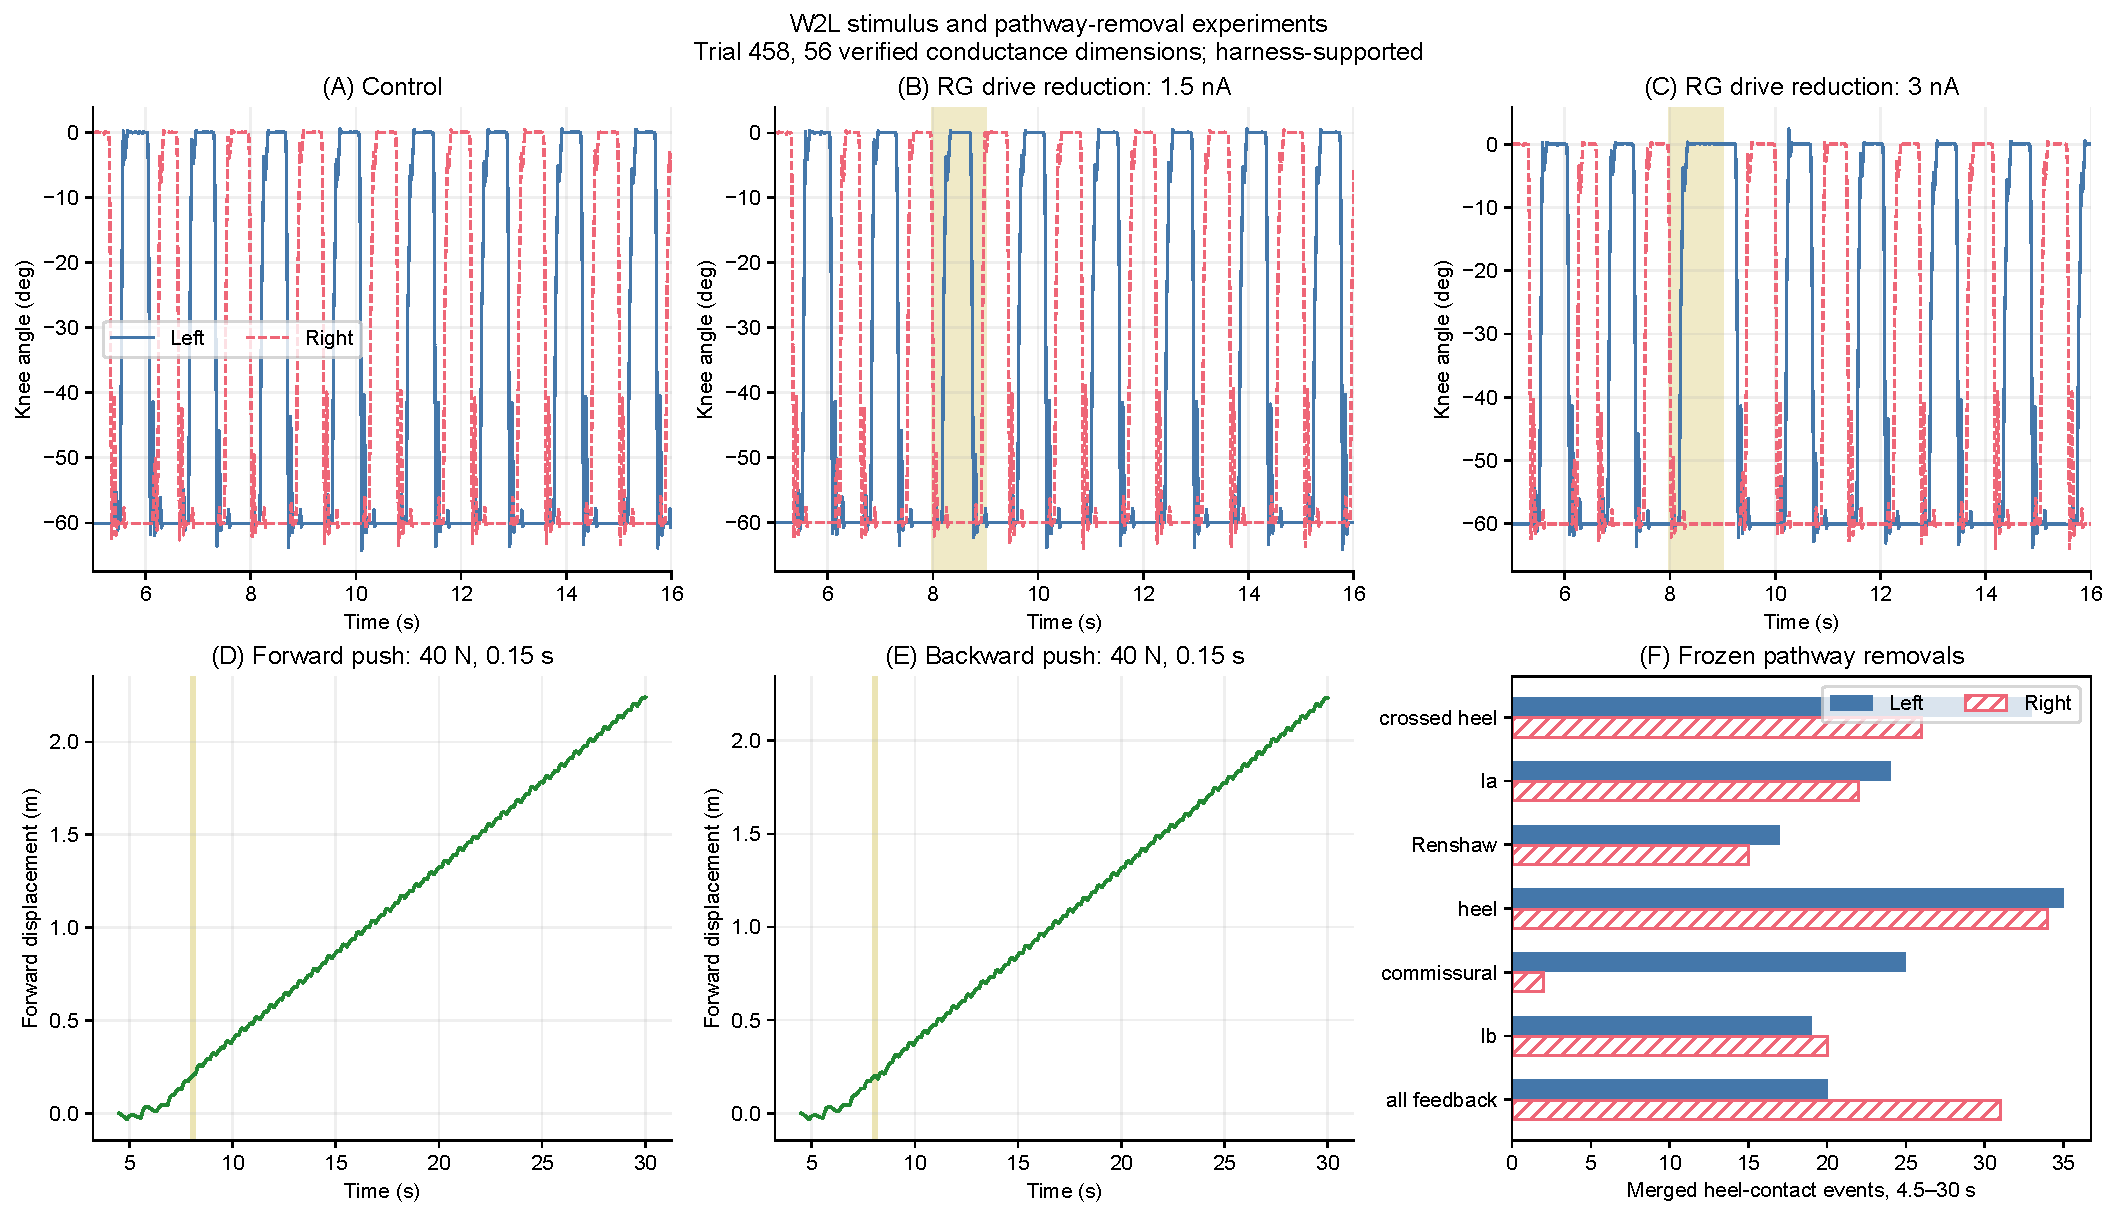
\includegraphics[width=\textwidth]{w2l_perturbation_verified.pdf}
\caption{Recovered W2L controller responses to drive changes, pushes, and pathway deletions. The same effective controller gains are used across conditions, with the specified intervention applied in each panel.}
\label{fig:app_w2l_perturbations}
\end{figure}

\subsection{Di Russo Controller Replication Attempt}\label{sec:app_dirusso_attempt}

The original Di Russo controller uses a reduced planar Delp/Thelen model with nine active coordinates and 18 Thelen muscles, rather than the full Gait2392 model. The source mechanical model loaded and its OpenSim system initialized successfully; this checks model construction, rather than gait. Its optimized parameter file contains 256 parameters, including individual reflex connections, muscle delays, and balance terms. Recovering that source clarified differences from the exploratory adaptation used here. Corrections to the adaptation addressed phase units, synchronous updates, output saturation, sensor ordering, contact-force direction, and initialization. Its compiled neural equations agreed with the corrected Python equations within $3.34\times10^{-16}$ over 2000 steps, establishing agreement between those two implementations.

A 960-trial exploratory duration-and-speed search nevertheless selected a tumbling trajectory, with pelvis rotation reaching approximately \ang{223}. That candidate was rejected as walking, and further optimization of the incomplete adaptation was stopped. The original controller's custom runtime was unavailable for a native baseline replay. The useful outcome is therefore the recovered source and the identified implementation requirements; replication of the published walking behavior remains incomplete. Source inventories, corrected-equation checks, and the rejected trajectory are retained in \nolinkurl{Code/MuJoCo_SNS/spinal/reports_20261027_codex/}.

\subsection{CAD-Derived Robot Integration}\label{sec:app_cad_supported_stance}

A separate CAD-derived robot model retained the four-bar knees and spherical hips, with 27 selected actuator routes per side. Its anatomical frame is $x$ anterior, $y$ superior, and $z$ right; explicit frame transformations distinguish it from older converted models. The controller drives simulated reference tensions rather than calibrated BPA forces, so this model does not yet validate the complete actuator-to-controller integration proposed in Chapter~\ref{ch:overall}.

The model completed a \qty{20}{\second} supported crouched-stance test. During the final five seconds, knee excursions were \ang{1.35} right and \ang{0.95} left, while the vertical rig carried \qty{94.68}{\percent} of body weight and angular stabilization remained active. Disabling muscle forces under the same support settings caused lumbar failure after \qty{0.202}{\second}. This comparison establishes a contribution of the muscle controller under strong assistance, not independent balance. A separate run with rhythmic drive completed its horizon, but alternating gait and progression after settling have not been verified.

A subsequent matched 40-second comparison retained the same geometry, initial pose, reference-tension capacities, and external assistance in both conditions. During 15--40 s, vertical assistance supplied 80\% of body weight. The additional control combines muscle-mediated separation feedback (160 N/m, capped at 20 N) with a 6\% activation floor on currently abducting routes, compared with the 5\% global floor (Table~\ref{tab:cad_abductor}). Full recorded trajectories reproduce bit for bit between fresh reference and accelerated runs. This is numerical replay within the specified model, rather than a robustness test.

\begin{table}[htbp]
\centering\small
\caption[Matched CAD-model separation-control comparison]{Matched CAD-model comparison over 15--40 s. Vertical assistance remains 80\% of body weight in both conditions.}
\label{tab:cad_abductor}
\begin{tabularx}{\textwidth}{@{}>{\raggedright\arraybackslash}Xrr@{}}
\toprule
Measure & Control off & Control on \\
\midrule
Reversed ankle ordering (\%) & 67 & 0 \\
Minimum ankle separation (mm) & $-38.3$ & 142.4 \\
Median ankle separation (mm) & $-6.2$ & 159.0 \\
Mean right TFL activation (\%) & 22.3 & 81.8 \\
Mean left TFL activation (\%) & 99.6 & 99.8 \\
Maximum sampled knee-loop error (mm) & 4.485 & 0.387 \\
Maximum sampled interleg penetration (mm) & 2.700 & 0 \\
\bottomrule
\end{tabularx}
\end{table}

The 262-neuron controller receives 230 inputs and drives 54 reference-tension actuators. Its MN target-current compensation cancels incoming PF and reflex synaptic currents to track the force allocator's targets. Consequently, the effective comparison concerns RG timing, engineered force allocation, and mechanical response, rather than normal PF/reflex authority over activation. Toe-out and small post-ramp knee excursions remain, and the stepping acceptance tests fail.

The foot attachment is an unverified assembly datum. A separate hypothesis translates each whole foot 60 mm toward the proximal shank, retaining tibial geometry and mass. With otherwise unchanged hybrid control, median ankle separation changes from 159.0 to \qty{57.3}{\milli\meter}, and sampled interleg penetration reaches \qty{1.316}{\milli\meter}. A separate W2L-organization timing probe has 544 neurons and 230 inputs; four named ankle indices alias knee-PF cells and are not additional neurons. Its shifted-foot condition passes bilateral unloading and lifting counts but fails repeated alternating foot apices and forward progression. The inherited MN compensation remains active, so this is not a full PF-driven controller comparison.

Route sites can lie outside CAD surfaces and transmit force through their named parent bodies, equivalent to ideal rigid offset brackets or guides. Bracket mass, compliance, packaging, and collision-aware wrapping remain unmodeled. These attachment assumptions are separate from verification of the source moving-point functions and complete path derivatives. The older 20-second stance test and newer 80\%-assistance comparison are different configurations, not a matched support-reduction experiment.

The W2L replay metrics and support accounting are archived in \nolinkurl{Code/MuJoCo_SNS/spinal/reports_20261027_codex/verification.json} and the accompanying support-ladder records. CAD-model stance metrics are in \nolinkurl{Code/MuJoCo_SNS/robot_torso/controller_assessment.json}. These records retain the configurations and evaluation conditions needed to distinguish the two models.


\section{OpenSim-to-MuJoCo Conversion Repairs}\label{sec:app_conversion_repairs}

The conversion work in Section~\ref{sec:sns_existing_tools} involved two distinct problems: importing the robot's artificial-muscle routing with human muscle parameters, and repairing the converted human reference used for controller development. The first combination failed muscle-equilibrium checks because the routed lengths were incompatible with the retained human parameters. The subsequent human-model repairs described below belong to that reference-model loading path; they are not evidence that the BPA-routed model reproduces every human muscle force.

\paragraph{Joint directions and coordinate conventions.}
Single-actuator tests exposed reversed hip-flexion and hip-adduction actions. The corresponding hinge-axis directions were negated so that the muscle actions agreed with the adopted OpenSim conventions. The knee required a different treatment: its converted flexion-negative convention was retained. Rotating the knee without updating its coupled translational coordinates gives a misleading geometry comparison, so those coordinates must follow the prescribed coupling during a pose or actuator test. These are specific joint and path checks, rather than a change from a left-handed to a right-handed model.

\paragraph{Small muscles and force scales.}
The quadratus femoris, gemelli, and piriformis actuators were disabled on both sides. Their six entries remain in the 92-actuator model, with no force contribution. A separate check found eight muscle-actuator entries with an active maximum-force scale of only \qty{1}{\newton}. Their active-force scales were restored from the source-model values. Table~\ref{tab:app_force_scale_repairs} lists the corrected values; each applies separately to the left and right actuator.

\begin{table}[htbp]
\centering
\caption{Active maximum-force scales restored in the converted human model.}
\label{tab:app_force_scale_repairs}
\begin{tabular}{@{}lrr@{}}
\toprule
Muscle & Converted scale (N) & Restored scale (N) \\
\midrule
Erector spinae & 1 & 2500 \\
Internal oblique & 1 & 900 \\
External oblique & 1 & 900 \\
Extensor hallucis longus & 1 & 162 \\
\bottomrule
\end{tabular}
\end{table}

These are source-model maximum-force parameters, not measured BPA capacities or the realized force at every pose. The passive-force scales already contained the source values. The converted length ranges for these entries remain a limitation, so restoring the active scale alone does not establish full force--length agreement.

\paragraph{Patella-related paths and coupled joints.}
The converted moving muscle-path points use joints coupled to knee angle. Their sampled limits conflicted with the coupling constraints away from the sampled pose, producing large constraint forces and restricted motion. The coupled path-point joints were therefore left without those conflicting limits while retaining their prescribed trajectories. The anatomical driver joints were treated separately: limits were re-enabled on 14 hinges using the converted ranges. The rectus femoris route also lacked the patella tracking needed for knee-extension action; its intermediate path point was replaced by the vastus medialis patella-tracking point. The force comparison below quantifies the remaining differences at matched poses and activations.

\paragraph{Contact and virtual geometry.}
The converted contact section contained 19 explicit ground--body pairs. These predefined pairs are independent of the individual geometry contact flags, so changing those flags alone did not remove ground contact in a suspended test. Suspended tests remove the explicit contact pairs; ground-contact tests retain only the six foot--ground pairs. Virtual muscle-path marker geometry was also prevented from colliding. This separates intended foot loading from unintended contact involving path markers or other body segments.

The repairs establish specific geometry, sign, constraint, and contact corrections. They do not remove the rigid-tendon approximation or establish complete equivalence with the OpenSim model. The appropriate result remains the corresponding test: correct muscle action, a valid coupled trajectory, intended ground contact, or agreement in the measured force comparison. None alone establishes walking performance.


\subsection{Cross-Platform Force Comparison}
\label{sec:muscle-models-compare}

The comparison script reads OpenSim static-optimization forces and activations and assigns the corresponding poses and activations to the converted MuJoCo model. It calls the forward calculation at each pose; it does not assign the trajectory velocities or integrate muscle activation and fiber dynamics through time. OpenSim static optimization likewise solves frame-by-frame force allocation rather than a compliant-tendon forward simulation \citep{opensim_static_optimization_docs}. The comparison therefore tests force predictions along sampled poses at matched activation, not dynamic equivalence or tendon-energy storage.

Table~\ref{tab:force-r2} retains the saved per-muscle statistics: $R^2=1-\mathrm{SSE}/\mathrm{SST}$, squared Pearson correlation, and the best-aligning lag in analysis frames. The calculation and saved values are in \nolinkurl{Code/MuJoCo_SNS/spinal/_muscle_force_compare.py} and \nolinkurl{muscle_force_compare.csv}.

\begin{table}[h]
  \centering
  \caption{MuJoCo vs.\ OpenSim muscle force along the subject01 walk at
  matched activations. Lag in analysis frames ($\approx 17$\,ms each).}
  \label{tab:force-r2}
  \small
  \begin{tabular}{lrrr}
    \toprule
    Muscle & $R^2$ & shape corr$^2$ & lag [frames] \\
    \midrule
    soleus   & 0.742 & 0.800 & 1 \\
    med.\ gastrocnemius & 0.888 & 0.894 & 2 \\
    lat.\ gastrocnemius & 0.884 & 0.887 & 2 \\
    tibialis anterior & 0.945 & 0.945 & 0 \\
    vastus lateralis & 0.941 & 0.945 & 1 \\
    rectus femoris & $-1.15$ & 0.384 & 0 \\
    semimembranosus & 0.565 & 0.621 & 0 \\
    biceps femoris short & $-0.26$ & 0.868 & 0 \\
    psoas & 0.927 & 0.934 & 1 \\
    gluteus maximus (2) & 0.926 & 0.943 & 1 \\
    tensor fasciae latae & 0.933 & 0.935 & 0 \\
    peroneus brevis & 0.977 & 0.989 & 0 \\
    \bottomrule
  \end{tabular}
\end{table}

Eight of the twelve representative muscles have $R^2$ between 0.87 and 0.98 and mean-force ratios within \qty{10}{\percent}. Soleus and semimembranosus have lower agreement, and the negative $R^2$ values for rectus femoris and biceps femoris short head indicate errors larger than predicting the corresponding mean reference force. Shape correlation alone does not remove those errors. The rectus femoris path was altered during conversion, while the biceps femoris short-head result has a substantial force-scale difference. These observations identify muscles requiring closer inspection; they do not isolate routing, force-law, and velocity effects from one another.

The frame-lag calculation describes alignment of these saved sequences. It cannot establish a physical delay caused by tendon compliance because the comparison does not simulate that mechanism. The results support selected pose-wise force checks, with the reported exceptions, rather than a general claim of equivalence for neural-control studies. A dynamic comparison would require matched velocities, activation histories, and explicitly specified tendon dynamics.

\begin{figure}[htbp]
  \centering
  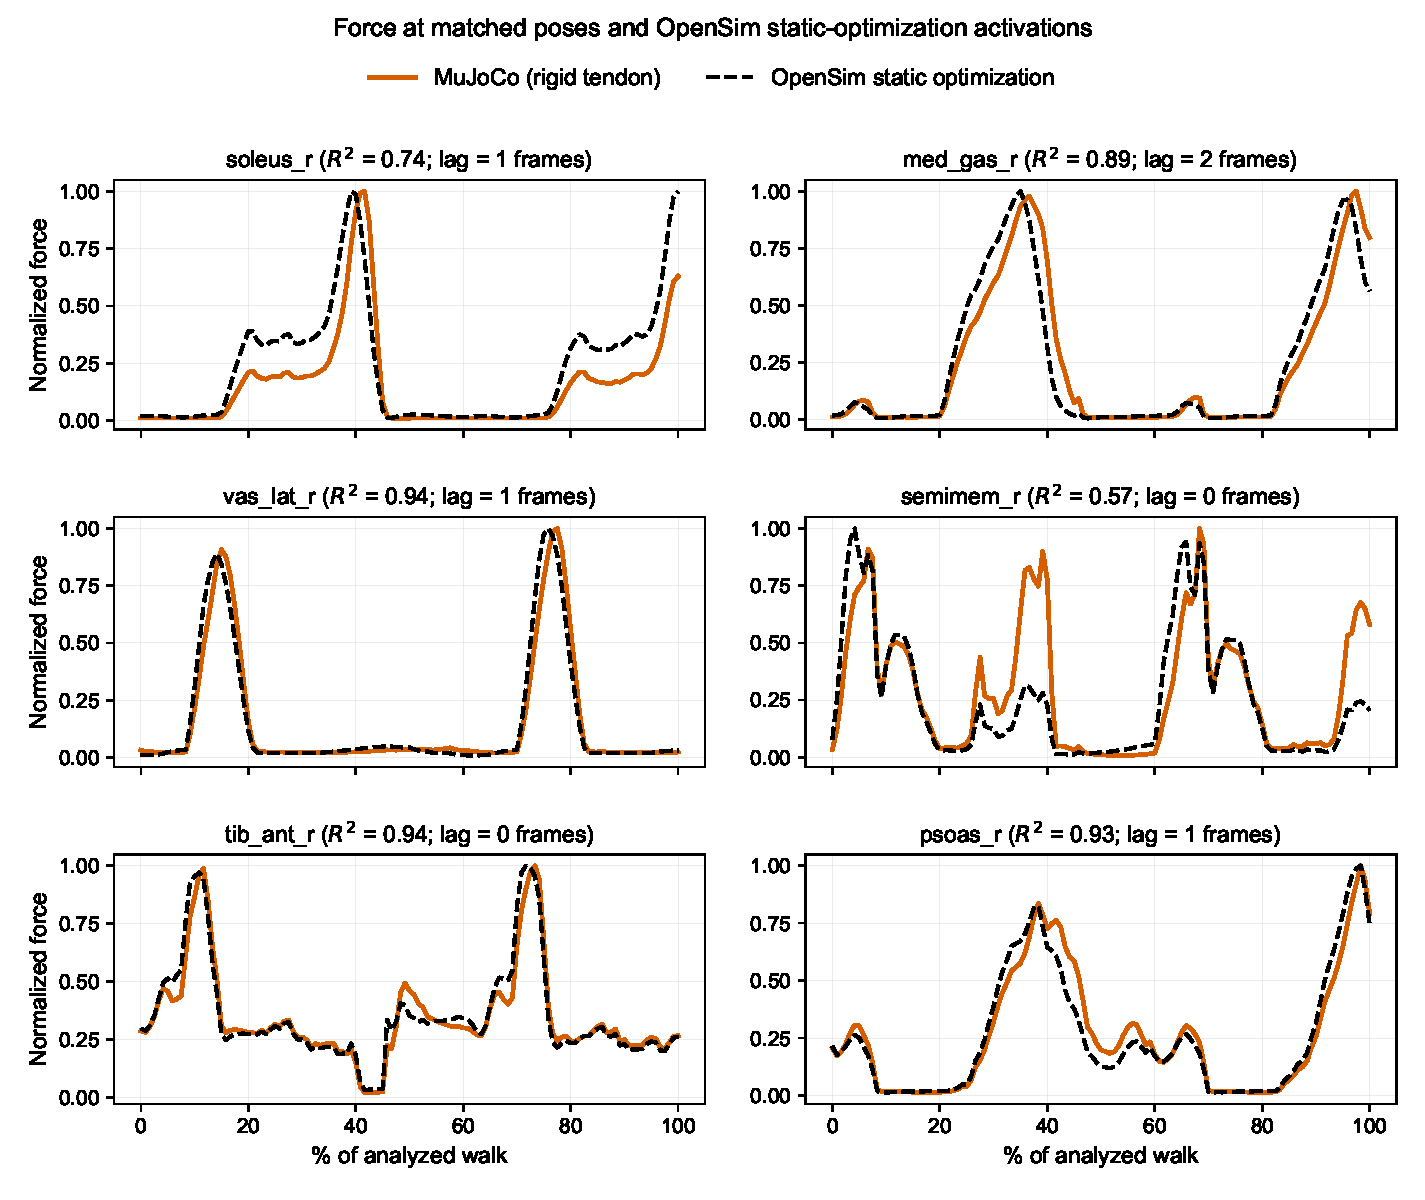
\includegraphics[width=0.9\textwidth]{muscle_force_compare_current.pdf}
  % ALT TEXT: Six-panel grid (three rows by two columns) of muscle
  % force versus time along the subject01 walk at matched activations,
  % one muscle per panel in reading order: soleus_r (top left),
  % med_gas_r, vas_lat_r, semimem_r, tib_ant_r, and psoas_r (bottom
  % right). Each panel overlays the MuJoCo rigid-tendon force (solid
  % orange) and the OpenSim static-optimization force (black
  % dashed), normalized to each muscle's own peak. Per-muscle R2,
  % shape correlation, lag, and force-ratio values for all twelve
  % analyzed muscles are archived in muscle_force_compare.csv beside
  % the figure file.
  \caption{Force sequences at matched poses and activations, normalized to each curve's peak. Absolute-force agreement is reported in Table~\ref{tab:force-r2}.}
  \label{fig:force-compare}
\end{figure}
